\section{Architecture}

\begin{figure}[h!]
  \centering
  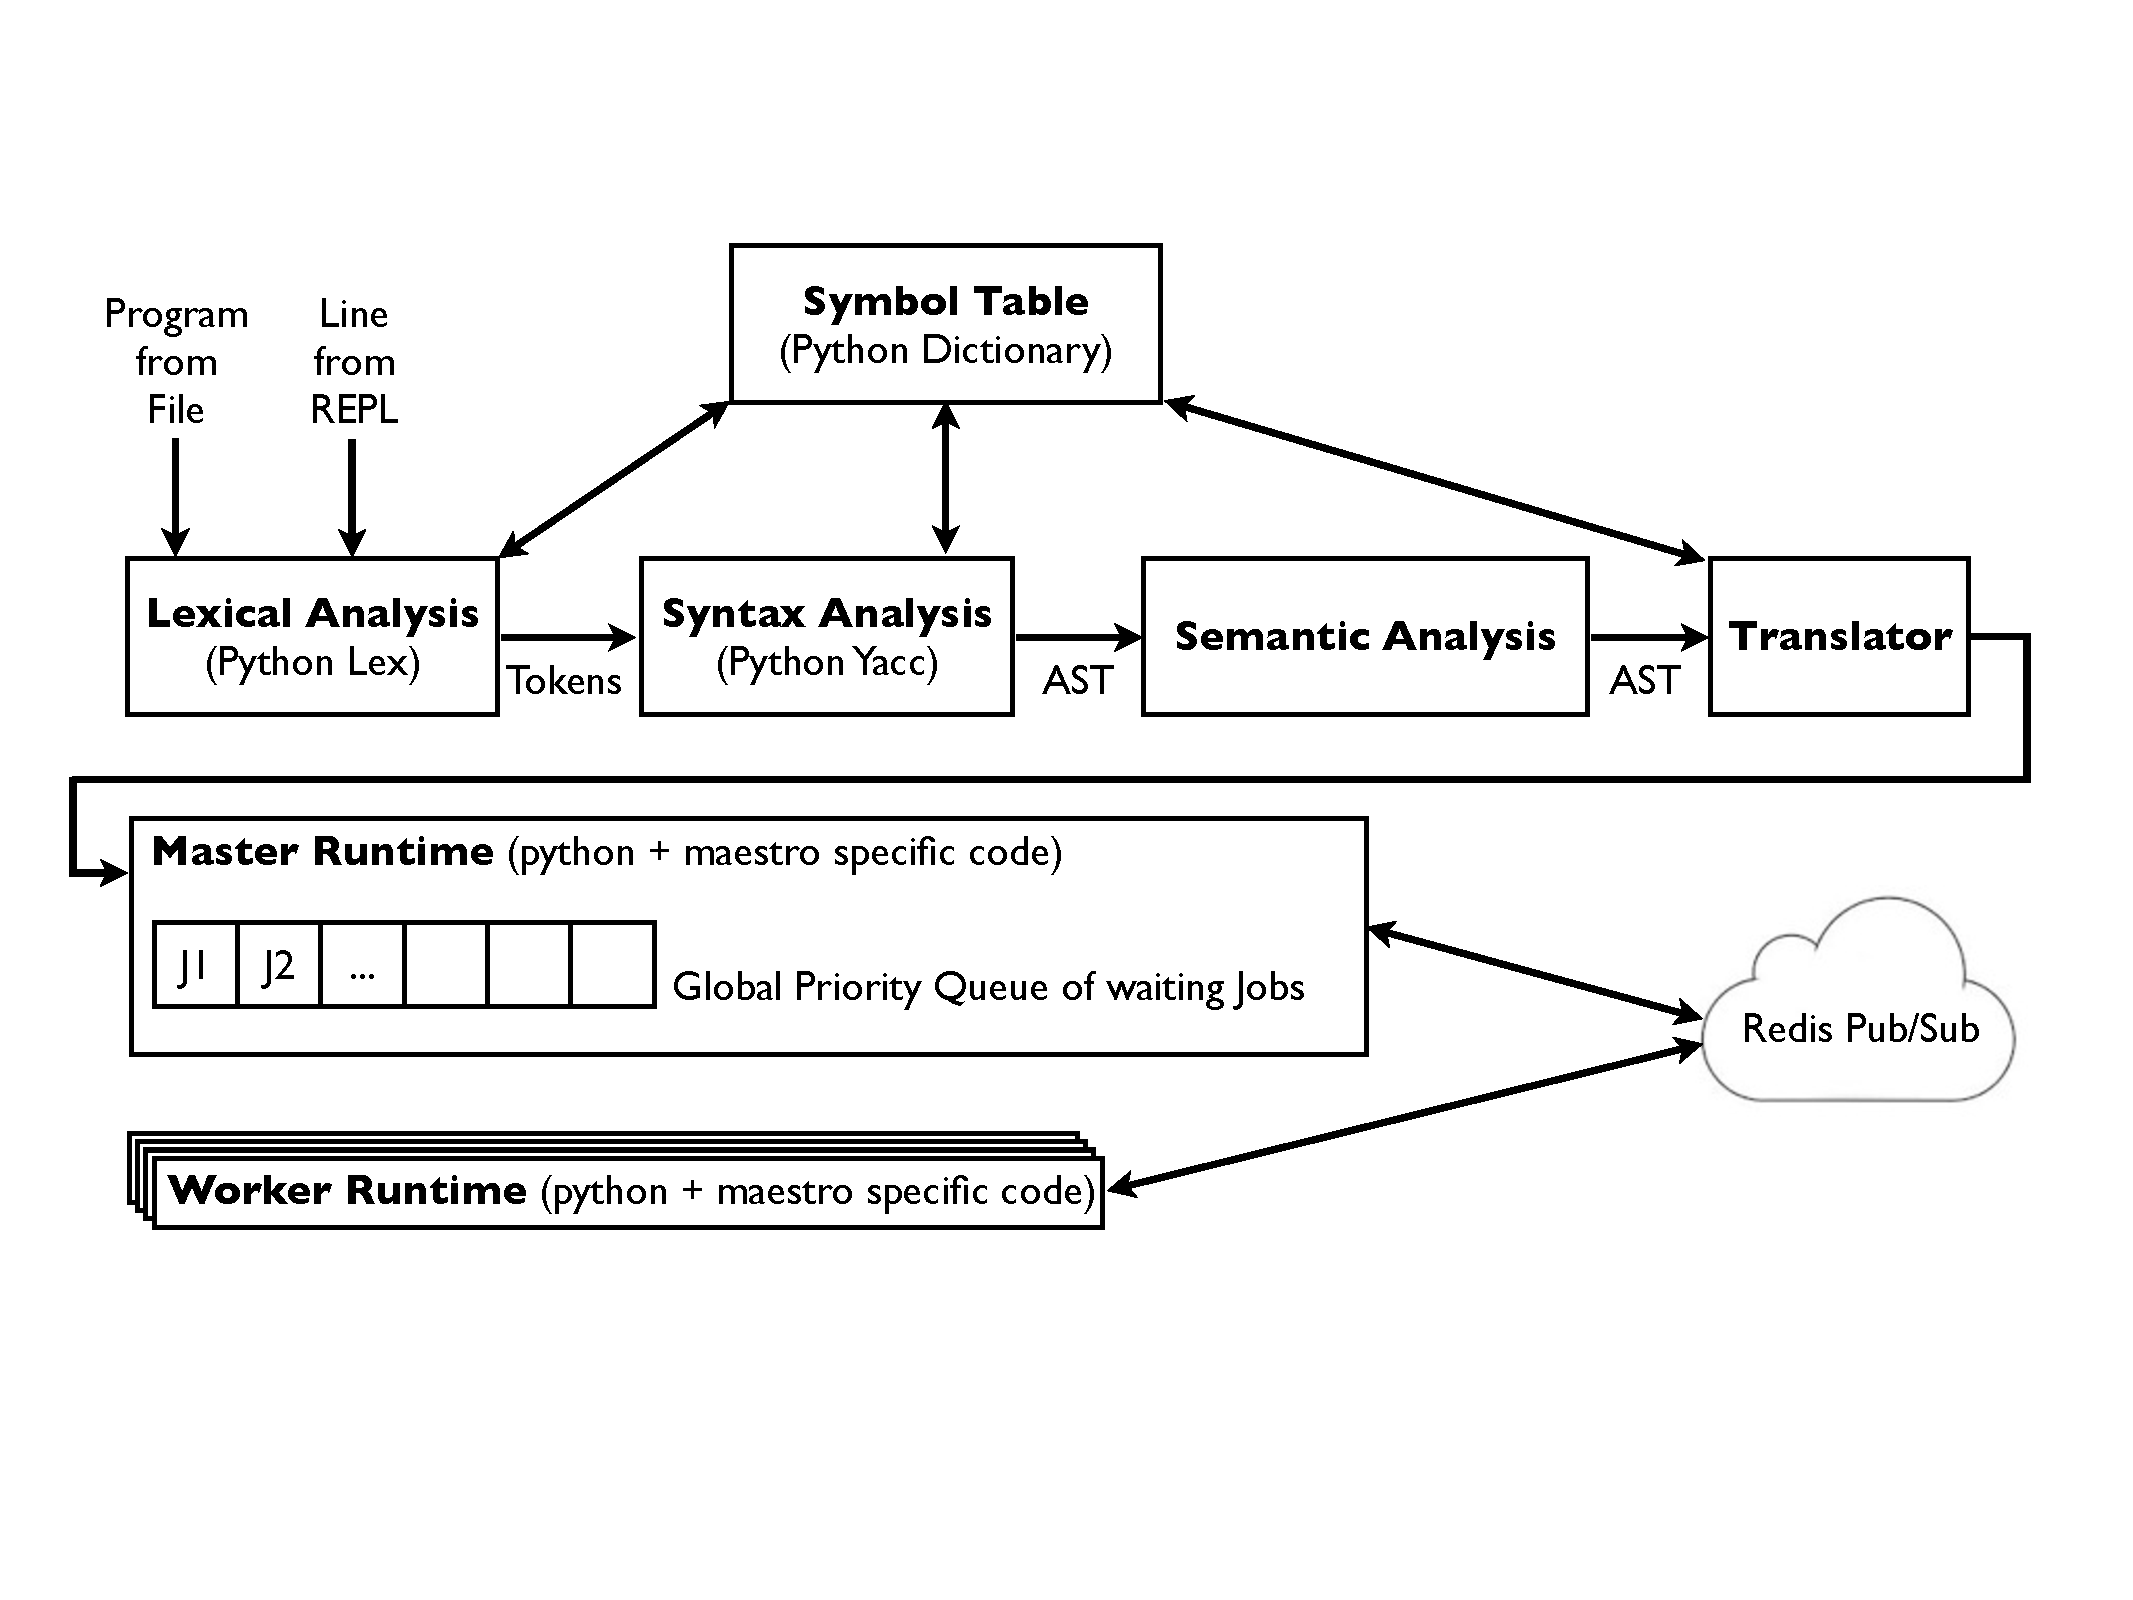
\includegraphics[width=15cm]{figures/archi.pdf}
  \caption{Maestro Architecture}
\end{figure}

\subsection{Interfaces}

\subsection{Modules}
Describe the interfaces between the modules.\\

State which modules were written by which team members.

\paragraph{Lexer (Mathias)}:
\paragraph{Syntax Analyser (Mathias)}:
\paragraph{Semantic Analyser (Georgios)}:
\paragraph{Translator (Mathias)}:
\paragraph{Backend (V. Atlidakis)} \newline
To support \lang{}'s job scheduling and dispatching for remote execution, we
built a distributed communication protocol whose main components are: (i)
a local job queue which in unique per runtime environment, (ii) a Redis
publish/subscribe communication channel, and (iii) a pool of workers dedicated
to job execution. The local job queue is used to keep track of active jobs
and their dependencies and is bind to a runtime environment. A custom Daemon
spins periodically on the job queue and dispatches for execution jobs with
resolved dependencies. Since job execution is either local or remote, job
dispatching is optional. On local execution, the job dispatcher requests a
shell on the local machine for job execution. On remote execution, the job
dispatcher sends a requests to check which are the active workers on the Redis
channel, and afterwards dispatches (publish) a job to the channel. One of the
subscribed active workers executes the job and sends back the output, on a job
specific redis channel. When the runtime Daemon receives the output of the
dispatched job via the job-specific channel, it prints its stdout and also
saves it in a log file under current working directory.

\paragraph{Testing (Arun and Yiren)}:

\section{Orgnaisation}
The hard thing with a multi-person project with many interacting parts is to figure out a way to all work in parallel.
We also wanted an early "hello world"...

To best achieve these objectives, 
